\documentclass[dvipdfmx]{ampbt}

%% クラスオプション:
%% chapter:   \chapterコマンドを使用可能にする(jsbook (report) を使う).
%% duplexing: 両面印刷用の PDF を出力する.
%% その他 jsclasses に指定可能なオプションが指定できます(そのまま渡される).

%% 報告書の題目 %%%%%%%%%%%%%%%%%%%%%%%%%%%%%%%%%%%%%%%%%%%%%%%%%%%%%%%%%%%%%%%%%
\title{数理モデルの構築と効率的なアルゴリズムの} % 題目1行目
      {開発に関する研究}                         % 題目2行目
      {}                                         % 題目3行目
%% 指導教員 %%%%%%%%%%%%%%%%%%%%%%%%%%%%%%%%%%%%%%%%%%%%%%%%%%%%%%%%%%%%%%%%%%%%%
\supervisors{情報太郎}{教授}    % 指導教員1人目 {氏名}{職名}
            {工学次郎}{助教}    % 指導教員2人目 {氏名}{職名}
            {}{}                % 指導教員3人目 {氏名}{職名}
%% 入学年月 %%%%%%%%%%%%%%%%%%%%%%%%%%%%%%%%%%%%%%%%%%%%%%%%%%%%%%%%%%%%%%%%%%%%%
\entrancedate{24}{4}            % {年(平成)}{月}
%% 著者氏名 %%%%%%%%%%%%%%%%%%%%%%%%%%%%%%%%%%%%%%%%%%%%%%%%%%%%%%%%%%%%%%%%%%%%%
\author{数理}{三郎}             % {姓}{名}
%% 提出日 %%%%%%%%%%%%%%%%%%%%%%%%%%%%%%%%%%%%%%%%%%%%%%%%%%%%%%%%%%%%%%%%%%%%%%%
\submissiondate{28}{1}{29}      % {年(平成)}{月}{日}
%% 提出年度 %%%%%%%%%%%%%%%%%%%%%%%%%%%%%%%%%%%%%%%%%%%%%%%%%%%%%%%%%%%%%%%%%%%%%
\submissionjay{27}              % {年度(平成)}
%% 摘要 %%%%%%%%%%%%%%%%%%%%%%%%%%%%%%%%%%%%%%%%%%%%%%%%%%%%%%%%%%%%%%%%%%%%%%%%%
\abstract{%
  本研究では,卒業論文を執筆する学生の数理モデルを構築し,このモデルを用いて効率
  的に卒業論文を作成するためのアルゴリズムを開発した.また,このアルゴリズムを用
  いて,実際に本報告を作成した.その結果,従来の自分で執筆する方法に比べて,65536
  倍効率的に卒業論文を作成することが可能であることが確認された.
}
%% パッケージの読み込みや自分用のマクロの定義 %%%%%%%%%%%%%%%%%%%%%%%%%%%%%%%%%%%
\usepackage{amsmath,amssymb}
\newcommand{\rme}{\mathrm{e}}

%% 出力の制御 %%%%%%%%%%%%%%%%%%%%%%%%%%%%%%%%%%%%%%%%%%%%%%%%%%%%%%%%%%%%%%%%%%%

%% 本文を出力しない場合,次の行をコメントアウトして下さい.
% \outputbodyfalse

%% 末尾に表紙,背表紙を出力しない場合,次の行をコメントアウトして下さい.
% \outputcoverfalse

%% 末尾に提出用摘要を出力しない場合,次の行をコメントアウトして下さい.
% \outputabstractforsubmissionfalse

%% ampbt.cls では表紙等の作成のために geometry パッケージを使用しているため,本文
%% のレイアウトを変えるために \usepackage[...]{geometry} とすると Option clash が
%% 発生します.何らかの理由で本文のレイアウトを変更したい場合は \geometry{...} を
%% 使用して下さい.
%% また,jsclasses を使用しているため,例えば 3cm を指定したい場合は 3truecm と書
%% く必要があります.
% \geometry{hmargin=3truecm,vmargin=2truecm}

\begin{document}
\ifoutputbody
%% 中表紙,摘要,目次 %%%%%%%%%%%%%%%%%%%%%%%%%%%%%%%%%%%%%%%%%%%%%%%%%%%%%%%%%%%
\makeinsidecover                % 中表紙
\makeabstract                   % 摘要
\maketoc                        % 目次
\setcounter{page}{1}            % 本文のページ番号を1から始める
%% 本文 %%%%%%%%%%%%%%%%%%%%%%%%%%%%%%%%%%%%%%%%%%%%%%%%%%%%%%%%%%%%%%%%%%%%%%%%%
\section{序論}
本研究では,卒業論文を執筆する学生の数理モデルを構築し,このモデルを用いて効率
的に卒業論文を作成するためのアルゴリズムを開発することを目的とする.
先行研究\cite{suuri2010}を改良し,より学生の実態に合致したモデルを構築する.
また,このアルゴリズムを用いて,実際に本報告を作成する実験を行う.

\section{数理モデルの構築}
本節では,学生と卒業論文の数理モデルを構築する.

\subsection{学生のやる気のモデル化}
時間を$t$とするとき,学生のやる気$x(t)$は,先行研究\cite{suuri2010}では次の式に従
うとされている:
\begin{equation}\label{eq:student}
  x(t)=x_0 \rme^{-t/a}.
\end{equation}
ここで,$x_0$は初期時刻$t=0$での学生のやる気,$a>0$は学生の研究への意欲を表す.
図~\ref{fig:student}はこのモデルによる学生のやる気の時間変化を$x_0=1$, $a=1$として
プロットしたものである.
\begin{figure}[htbp]
  \centering
  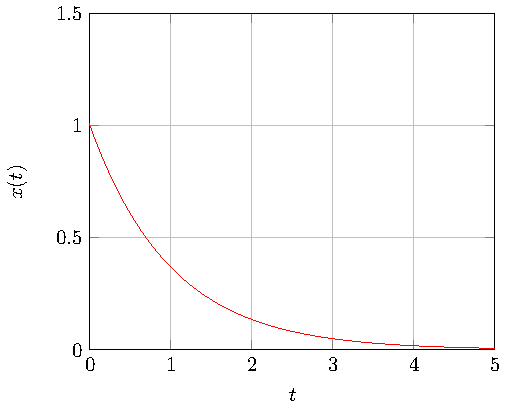
\includegraphics{ampbt_figure.pdf}
  \caption{モデル\eqref{eq:student}による$x_0=1$, $a=1$のときの学生のやる気の時間
    変化.}
  \label{fig:student}
\end{figure}

モデル\eqref{eq:student}については,次のような問題点がある.
\begin{itemize}
\item 研究の進み具合や休憩によってやる気が復活する効果が考慮されていない.
\item 締切が迫ってきたときのラストスパートが反映されていない.
\end{itemize}

以上の問題点を踏まえて,次のような改良を考える.
…….

\subsection{卒業論文のモデル化}
…….

\section{効率的なアルゴリズムの開発}
本節では,前節までの結果を用いて,効率的に卒業論文を作成するためのアルゴリズムを開
発する.
…….

\section{結論}
本研究では,卒業論文を執筆する学生の数理モデルを構築した.
また,このモデルを用いて効率的に卒業論文を作成するためのアルゴリズムを開発し,実際
にこのアルゴリズムを用いて本報告を作成する実験を行った.その結果,従来の自分で執筆
する方法に比べて,65536倍効率的に卒業論文を作成することが可能であることが確認され
た.

今後の課題としては,修士論文や学術誌への投稿論文にもこのアルゴリズムを適用すること
が考えられる.

%% 謝辞 %%%%%%%%%%%%%%%%%%%%%%%%%%%%%%%%%%%%%%%%%%%%%%%%%%%%%%%%%%%%%%%%%%%%%%%%%
\acknowledgment
本研究に取り組むにあたって助言をいただいた情報太郎教授と工学次郎助教に深く感謝
する.

%% 参考文献 %%%%%%%%%%%%%%%%%%%%%%%%%%%%%%%%%%%%%%%%%%%%%%%%%%%%%%%%%%%%%%%%%%%%%
\addcontentsline{toc}{section}{\refname} % 目次に参考文献を追加する.
                                         % chapter使用時は削除すること.
\begin{thebibliography}{10}
\bibitem{polya1945}
  G.~Polya, \textit{How to solve it: a new aspect of mathematical method},
  Princeton University Press, Princeton, 1945.
\bibitem{suuri2010}
  数理花子,数理モデルとその妥当性の検討,
  京都大学工学部情報学科数理工学コース特別研究報告,2010.
\end{thebibliography}
%% BibTeX 等を用いる場合は,上の thebibliography 環境を消してここに該当コードを
%% 挿入すること.
% \bibliographystyle{...}
% \bibliography{...}

%% 付録 %%%%%%%%%%%%%%%%%%%%%%%%%%%%%%%%%%%%%%%%%%%%%%%%%%%%%%%%%%%%%%%%%%%%%%%%%
%% 付録は不要ならば削除してよい.
\appendix

\section{意味のない付録}
これは意味のない付録です.これは意味のない引用です\cite{polya1945}.

\begin{table}[htbp]
  \caption{これは意味のない表です.}
  \centering
  \begin{tabular}{c|cc}
      &  A  &  B \\
    \hline
    C &  70 & 80 \\
    D & 100 &  0
  \end{tabular}
\end{table}

%% 本文ここまで %%%%%%%%%%%%%%%%%%%%%%%%%%%%%%%%%%%%%%%%%%%%%%%%%%%%%%%%%%%%%%%%%
\fi
\ifoutputcover
\evenclearpage
%% 表紙,背表紙,提出用摘要 %%%%%%%%%%%%%%%%%%%%%%%%%%%%%%%%%%%%%%%%%%%%%%%%%%%%%
\makecover                      % 表紙
\makespine[1]                   % 背表紙([] 内は出力枚数)
\makeinsidecover                % 中表紙
\fi
\ifoutputabstractforsubmission
\makeabstractforsubmission      % 提出用摘要
\fi
\end{document}
